\section{HAM10000}
\label{sec:data-ham}

All experiments use HAM10000~\cite{tschandl2018ham10000}, obtained from Harvard
Dataverse~\cite{tschandl2018ham10000_dataverse} rather than from a mirror, so the
provenance is citable. The archive supplies 10{,}015 dermatoscopic images in two parts
together with a metadata table.

Two practical details about that distribution are worth recording, because both will
break a loader written against the more common Kaggle layout. The images arrive as two
ZIP archives with the JPEGs at the root rather than inside named folders, and the
metadata file is called \texttt{HAM10000\_metadata} with no file extension despite
containing ordinary comma-separated values. Both are handled explicitly in the data
preparation notebook.

The metadata provides seven fields, of which three matter here: \texttt{lesion\_id},
\texttt{image\_id} and \texttt{dx}. The remaining fields (\texttt{dx\_type},
\texttt{age}, \texttt{sex}, \texttt{localization}) are not used as model inputs. Every
image is classified into one of seven diagnostic categories, listed in
Table~\ref{tab:classes}.

\begin{table}[htbp]
\centering
\caption{The seven diagnostic categories in HAM10000, with observed counts.}
\label{tab:classes}
\small
\begin{tabular}{@{}llrrl@{}}
\toprule
\textbf{Code} & \textbf{Diagnosis} & \textbf{Images} & \textbf{Share} & \textbf{Nature} \\
\midrule
nv    & Melanocytic nevi                  & 6{,}705 & 66.95\% & Benign \\
mel   & Melanoma                          & 1{,}113 & 11.11\% & \textbf{Malignant} \\
bkl   & Benign keratosis-like lesions     & 1{,}099 & 10.97\% & Benign \\
bcc   & Basal cell carcinoma              &    514 &  5.13\% & \textbf{Malignant} \\
akiec & Actinic keratoses / Bowen's       &    327 &  3.27\% & Pre-malignant \\
vasc  & Vascular lesions                  &    142 &  1.42\% & Benign \\
df    & Dermatofibroma                    &    115 &  1.15\% & Benign \\
\midrule
      & \textbf{Total}                    & \textbf{10{,}015} & 100\% & \\
\bottomrule
\end{tabular}
\end{table}

\section{The Imbalance Problem, Quantified}
\label{sec:data-imbalance}

The distribution in Table~\ref{tab:classes} is severely long-tailed. Melanocytic nevi
outnumber dermatofibroma by 58.3 to 1. Figure~\ref{fig:class-dist} shows the shape.

\begin{figure}[htbp]
\centering
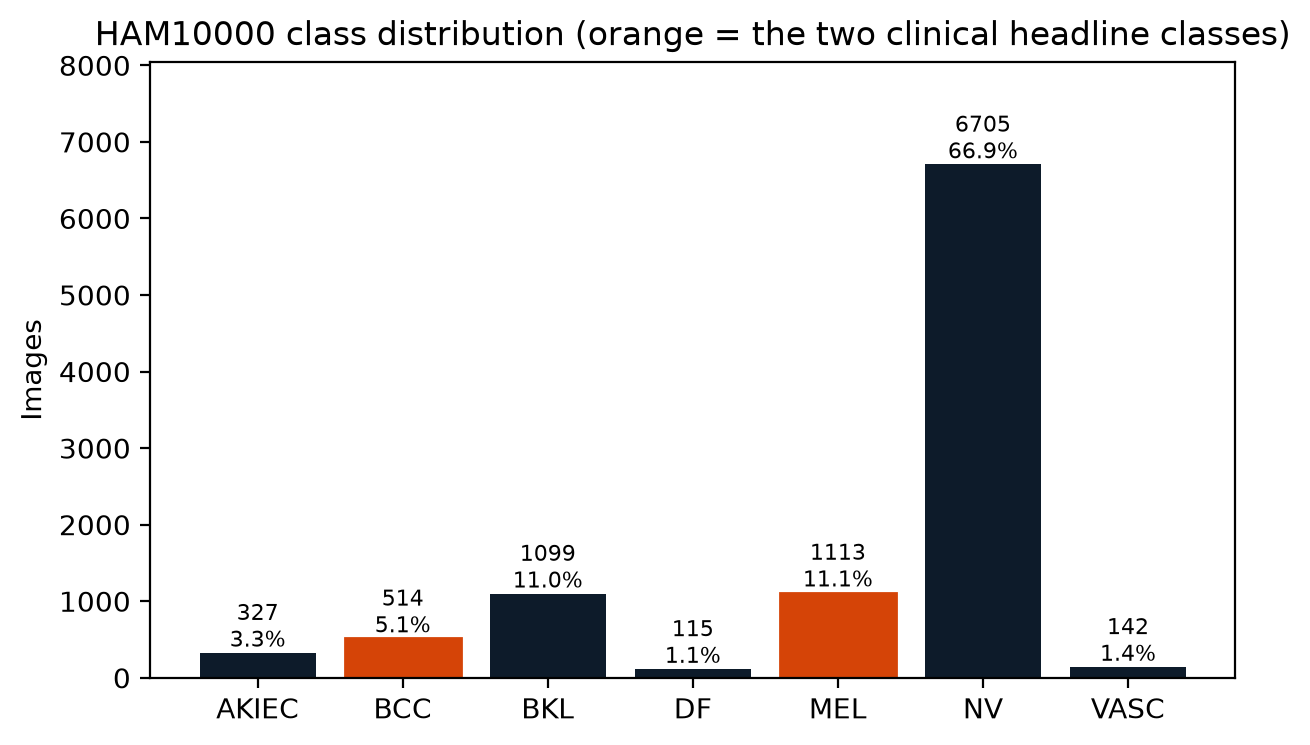
\includegraphics[width=0.85\textwidth]{figures/eda_class_distribution.png}
\caption{Class distribution across the full dataset. The two clinically significant
classes, melanoma and basal cell carcinoma, are highlighted. Together they account for
16.2\% of the data while carrying essentially all of the clinical risk.}
\label{fig:class-dist}
\end{figure}

The consequence is worth stating as a number rather than a warning. A classifier that
ignores its input entirely and answers \emph{nevus} every time achieves:

\begin{equation}
  \frac{6{,}705}{10{,}015} = 66.95\%\ \text{accuracy}
  \label{eq:naive}
\end{equation}

while detecting none of the 1{,}113 melanomas. That figure is not far below much of the
accuracy reported in the HAM10000 literature. It is the reason this thesis treats
overall accuracy as a diagnostic of dataset composition rather than of model quality,
and reports per-class F1 as the primary metric instead.

\section{Lesion-Level Splitting}
\label{sec:data-split}

HAM10000 photographs many lesions more than once. Of the 7{,}470 distinct lesions in the
set, 1{,}956 contribute more than one image. Multiple photographs of the same lesion are
near-duplicates: same patient, same site, same session, differing mainly in framing and
illumination.

Splitting on \texttt{image\_id} would therefore place near-identical images on both
sides of the train/test boundary. The resulting test accuracy would partly measure
memorisation of specific lesions rather than generalisation to new ones, and it would be
inflated in a way that no amount of careful metric selection afterwards could detect.

The split is therefore performed on \texttt{lesion\_id}, so every photograph of a given
lesion lands in exactly one partition. It is stratified by diagnosis to preserve class
proportions, uses an 80/10/10 ratio, and is seeded at 42.

\begin{table}[htbp]
\centering
\caption{Partition sizes. The split is computed over lesions; image counts follow from
which lesions land where, which is why the image ratios are not exactly 80/10/10.}
\label{tab:split-sizes}
\small
\begin{tabular}{@{}lrrr@{}}
\toprule
\textbf{Partition} & \textbf{Lesions} & \textbf{Images} & \textbf{Share of images} \\
\midrule
Train & 5{,}976 & 8{,}012 & 80.0\% \\
Validation &   747 &   979 &  9.8\% \\
Test  &   747 & 1{,}024 & 10.2\% \\
\midrule
\textbf{Total} & \textbf{7{,}470} & \textbf{10{,}015} & 100\% \\
\bottomrule
\end{tabular}
\end{table}

The split is computed once, written to
\texttt{runs/splits/seed42\_lesion\_stratified.json}, and hashed. Every subsequent run
loads that file rather than recomputing, and records the hash in its own
\texttt{config.json}. The hash for all runs reported in this thesis is
\texttt{f35ac1de18678182}. A run that somehow saw different data would carry a different
hash and be immediately identifiable, which converts an assumption into a check.

\subsection{Leakage verification}

Two assertions are executed in the data preparation notebook and must both hold before
any training begins. No \texttt{lesion\_id} may appear in more than one partition, and
no \texttt{image\_id} may appear in more than one partition. The second follows from the
first but is checked independently, because it is the property that actually matters and
a bug in the lesion-to-image mapping would violate it while leaving the first intact.
Both pass with zero overlaps.

\subsection{Stratification quality}

Table~\ref{tab:split-class} gives the resulting per-class distribution. Proportions are
preserved to within roughly one percentage point in every class.

\begin{table}[htbp]
\centering
\caption{Class composition of each partition. Test-set support is the figure that
matters when reading per-class metrics in Chapter~7.}
\label{tab:split-class}
\small
\begin{tabular}{@{}lrrrrrr@{}}
\toprule
& \multicolumn{2}{c}{\textbf{Train}} & \multicolumn{2}{c}{\textbf{Validation}}
& \multicolumn{2}{c}{\textbf{Test}} \\
\cmidrule(lr){2-3}\cmidrule(lr){4-5}\cmidrule(lr){6-7}
\textbf{Class} & $n$ & \% & $n$ & \% & $n$ & \% \\
\midrule
nv    & 5{,}354 & 66.8 & 661 & 67.5 & 690 & 67.4 \\
mel   &    892 & 11.1 & 106 & 10.8 & 115 & 11.2 \\
bkl   &    896 & 11.2 &  98 & 10.0 & 105 & 10.3 \\
bcc   &    403 &  5.0 &  58 &  5.9 &  53 &  5.2 \\
akiec &    261 &  3.3 &  33 &  3.4 &  33 &  3.2 \\
vasc  &    115 &  1.4 &  12 &  1.2 &  15 &  1.5 \\
df    &     91 &  1.1 &  11 &  1.1 &  13 &  1.3 \\
\midrule
\textbf{Total} & \textbf{8{,}012} & & \textbf{979} & & \textbf{1{,}024} & \\
\bottomrule
\end{tabular}
\end{table}

The test-set support figures deserve attention when reading later results. Melanoma has
115 test images and basal cell carcinoma has 53, so per-class metrics for those classes
are computed over samples of that size. Dermatofibroma has 13. A single additional
correct prediction moves dermatofibroma recall by roughly 7.7 percentage points, and
per-class figures for the rarest classes should be read with that granularity in mind.

\section{Class Weights}
\label{sec:data-weights}

The weighted cross-entropy condition uses inverse-frequency weights computed on the
training partition:

\begin{equation}
  w_c = \frac{N}{K \cdot n_c}
  \label{eq:weights}
\end{equation}

where $N = 8{,}012$ is the training set size, $K = 7$ is the number of classes, and
$n_c$ is the count of class $c$ in training. Table~\ref{tab:weights} gives the resulting
values.

\begin{table}[htbp]
\centering
\caption{Inverse-frequency class weights on the training partition.}
\label{tab:weights}
\small
\begin{tabular}{@{}lrr@{}}
\toprule
\textbf{Class} & \textbf{Train $n$} & \textbf{Weight $w_c$} \\
\midrule
nv    & 5{,}354 &  0.214 \\
bkl   &    896 &  1.277 \\
mel   &    892 &  1.283 \\
bcc   &    403 &  2.840 \\
akiec &    261 &  4.385 \\
vasc  &    115 &  9.953 \\
df    &     91 & 12.578 \\
\midrule
\multicolumn{2}{@{}l}{\textbf{Ratio, largest to smallest}} & \textbf{58.8} \\
\bottomrule
\end{tabular}
\end{table}

A spread of 58.8 to 1 is large. A dermatofibroma training example contributes almost
sixty times the gradient signal of a nevus example. This is the intended behaviour of
inverse-frequency weighting, but it is an aggressive intervention rather than a neutral
correction, and Chapter~8 returns to what it does to the runs that use it.

\section{Preprocessing}
\label{sec:data-preproc}

Images are stored at $600 \times 450$ pixels. All are resized to the square input
expected by the network, 224 pixels for the confirmatory runs and the matched-resolution
ablation, 300 pixels for the native-resolution ablation, and normalised with ImageNet
channel statistics~\cite{russakovsky2015imagenet} since all three backbones start from
ImageNet-pretrained weights.

Training images additionally receive random horizontal flip, random vertical flip,
rotation within $\pm 30^{\circ}$, and colour jitter on brightness, contrast and
saturation. Both flips are appropriate here because dermatoscopic images have no
canonical orientation: a lesion photographed upside down is the same lesion. Colour
jitter is bounded at 0.2 on each channel, deliberately modest, since colour carries
genuine diagnostic information in dermatology and aggressive jitter would destroy signal
rather than add invariance.

Validation and test images receive resize and normalisation only. No augmentation is
applied at evaluation time, and no test-time augmentation is used anywhere in this
thesis.
